\documentclass[xetex,mathserif,serif]{beamer}
\usepackage{polyglossia}
\setdefaultlanguage[babelshorthands=true]{russian}
\usepackage{minted}
\usepackage{tabu}
\usepackage{forest}

\usepackage{textpos}
\setlength{\TPHorizModule}{1cm}
\setlength{\TPVertModule}{1cm}

\usetikzlibrary{arrows}

\useoutertheme{infolines}

\setmainfont{FreeSans}
\newfontfamily{\russianfonttt}{FreeSans}

\definecolor{links}{HTML}{2A1B81}
\hypersetup{colorlinks,linkcolor=,urlcolor=links}

\tabulinesep=1.2mm

\newcommand{\attribution}[1] {
	\begin{flushright}\begin{scriptsize}\textcolor{gray}{\textcopyright\, #1}\end{scriptsize}\end{flushright}
}

\title{Сортировки и поиск}
\author[Юрий Литвинов]{Юрий Литвинов \newline \textcolor{gray}{\small\texttt{yurii.litvinov@gmail.com}}}
\date{02.03.2018г}

\begin{document}
	
	\frame{\titlepage}

	\begin{frame}
		\frametitle{Свойства алгоритмов сортировки}
		\begin{itemize}
			\item Работают над любыми контейнерами данных
			\item Есть понятие ``ключ''
			\item Устойчивость --- сохраняется ли взаимное расположение элементов с одинаковым ключом
			\item Естественность --- учёт степени отсортированности исходных данных
			\item Внутренняя сортировка --- работает над данными, целиком помещающимися в память
			\item Внешняя сортировка работает над данными на устройствах с последовательным доступом, которые медленнее, чем память
		\end{itemize}
	\end{frame}

	\begin{frame}
		\frametitle{Сортировка пузырьком (bubble sort)}
		\begin{columns}
			\begin{column}{0.25\textwidth}
			\end{column}
			\begin{column}{0.75\textwidth}
				\begin{itemize}
					\item
				\end{itemize}
			\end{column}
		\end{columns}
	\end{frame}

	\begin{frame}
		\frametitle{Сортировка выбором (selection sort)}
		\begin{columns}
			\begin{column}{0.25\textwidth}
				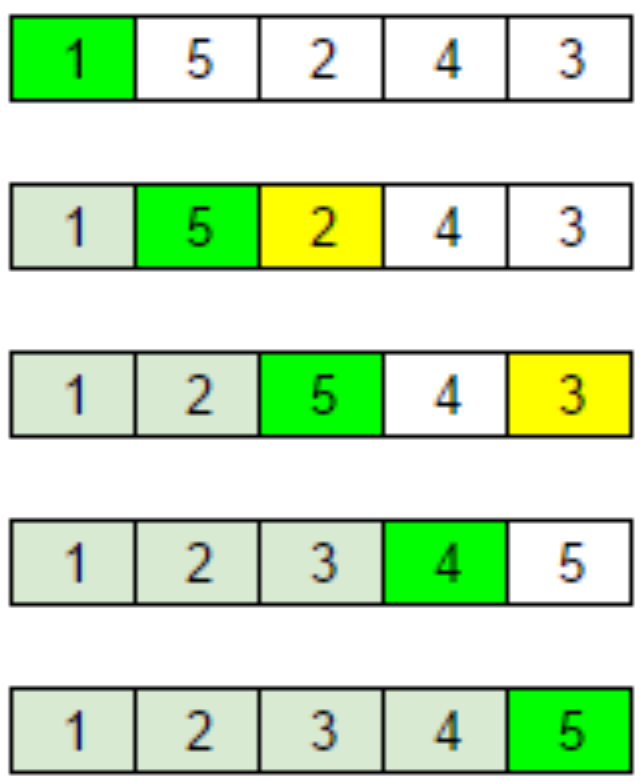
\includegraphics[width=\textwidth]{selectSort.png}
			\end{column}
			\begin{column}{0.75\textwidth}
				\begin{itemize}
					\item $O(n^2)$
					\item Обычно неустойчива ($[2_a, 2_b, 1_a] -> [1_a, 2_b, 2_a]$)
					\item Отсортированность массива ничего не даёт
					\item Меньше всего операций обмена (меньше операций записи, что иногда позитивно)
					\item \url{https://www.ee.ryerson.ca/~courses/coe428/sorting/selectionsort.html}
				\end{itemize}
			\end{column}
		\end{columns}
	\end{frame}

	\begin{frame}
		\frametitle{Сортировка вставкой (insertion sort)}
		\begin{columns}
			\begin{column}{0.25\textwidth}
				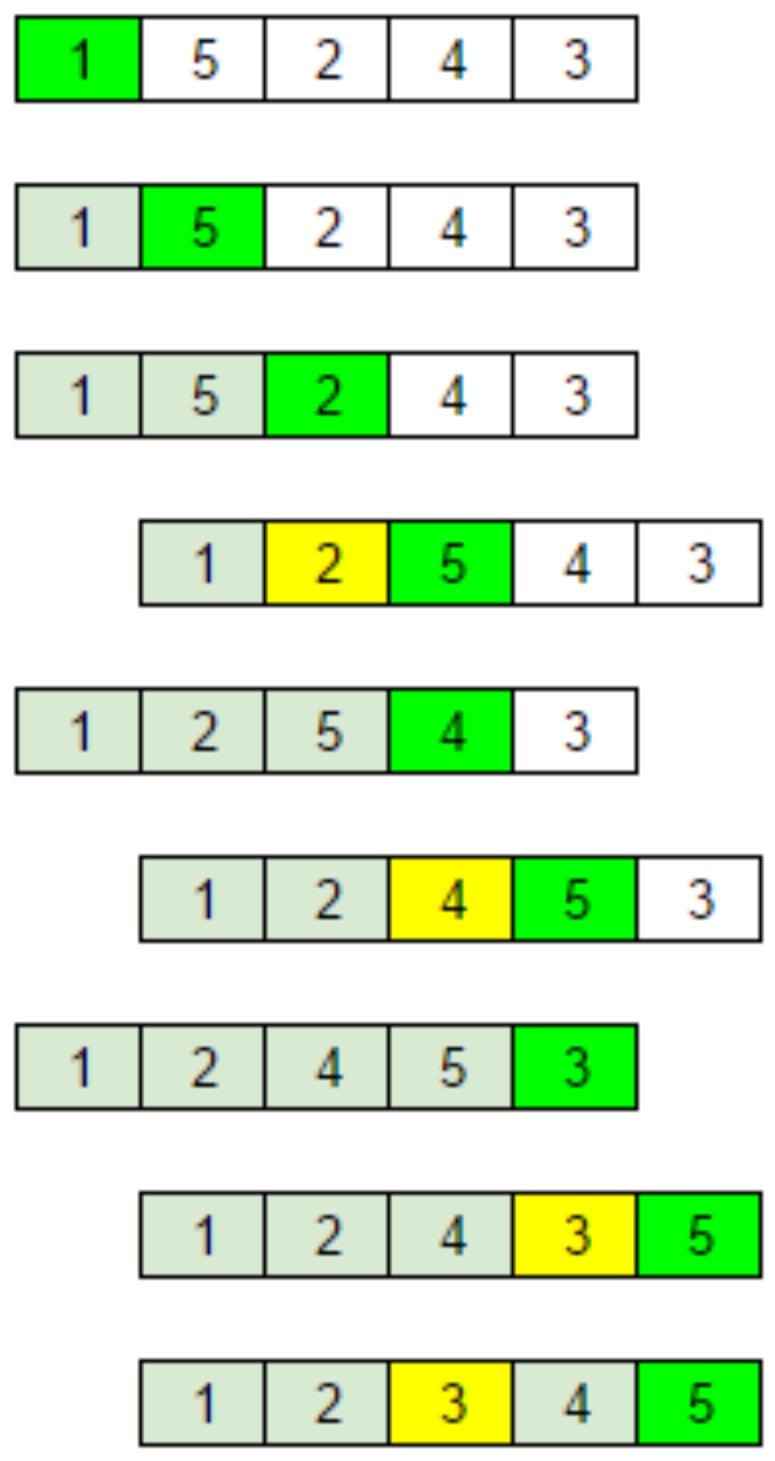
\includegraphics[width=\textwidth]{insertSort.png}
			\end{column}
			\begin{column}{0.75\textwidth}
				\begin{itemize}
					\item $O(n^2)$
					\item Устойчива
					\item Естественная ($O(n)$ на отсортированном массиве)
					\item Данные могут приходить постепенно
					\item Позволяет выбрать наибольшие (или наименьшие) k чисел из входного потока
					\item \url{https://www.ee.ryerson.ca/~courses/coe428/sorting/insertionsort.html}
				\end{itemize}
			\end{column}
		\end{columns}
	\end{frame}

	\begin{frame}
		\frametitle{Сортировка Шелла (Shell sort)}
		\begin{columns}
			\begin{column}{0.35\textwidth}
				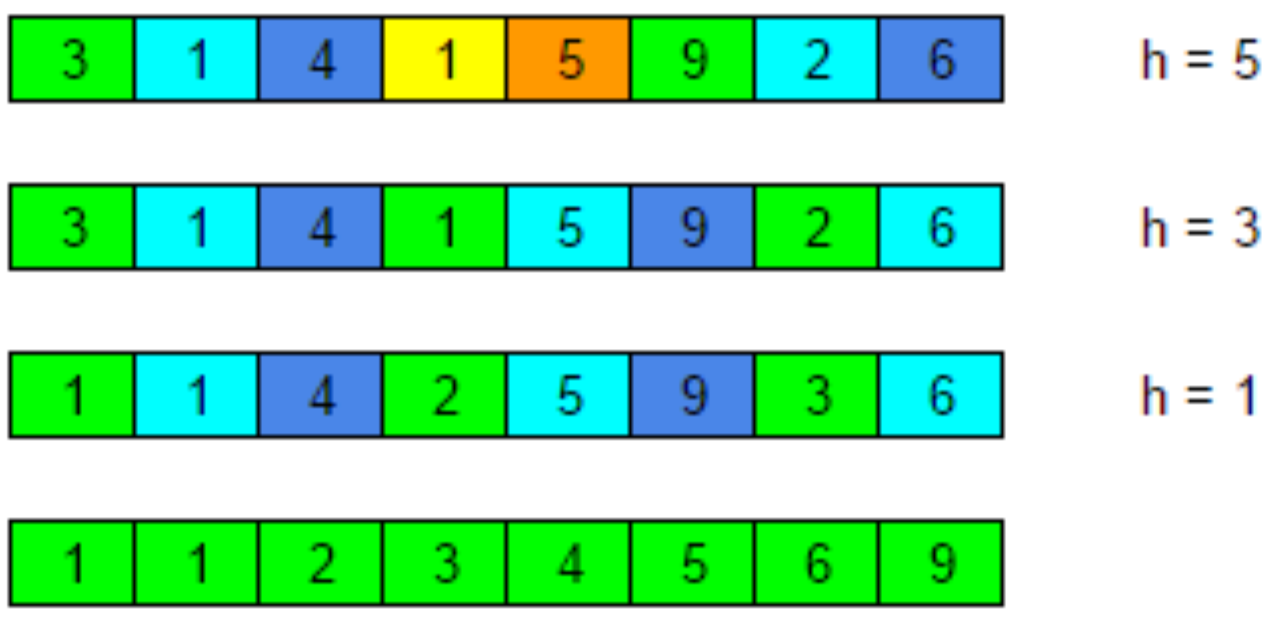
\includegraphics[width=\textwidth]{shellSort.png}
			\end{column}
			\begin{column}{0.65\textwidth}
				\begin{itemize}
					\item Сортировка вставкой подпоследовательностей в массиве с постепенно убывающим шагом
					\item Элементы ``быстрее'' встают на свои места
					\begin{itemize}
						\item Сортировка вставкой на каждом шаге уменьшает количество инверсий максимум на 1
					\end{itemize}
					\item $O(n * log(n)^2)$ при правильном выборе h
					\item Неустойчива
					\item Легко пишется и довольно быстра
					\begin{itemize}
						\item Не вырождается до квадратичной
					\end{itemize}
				\end{itemize}
			\end{column}
		\end{columns}
	\end{frame}

	\begin{frame}
		\frametitle{Сортировка подсчётм (counting sort)}
		\begin{columns}
			\begin{column}{0.25\textwidth}
			\end{column}
			\begin{column}{0.75\textwidth}
				\begin{itemize}
					\item
				\end{itemize}
			\end{column}
		\end{columns}
	\end{frame}

	\begin{frame}
		\frametitle{Быстрая сортировка (qsort)}
		\begin{columns}
			\begin{column}{0.5\textwidth}
				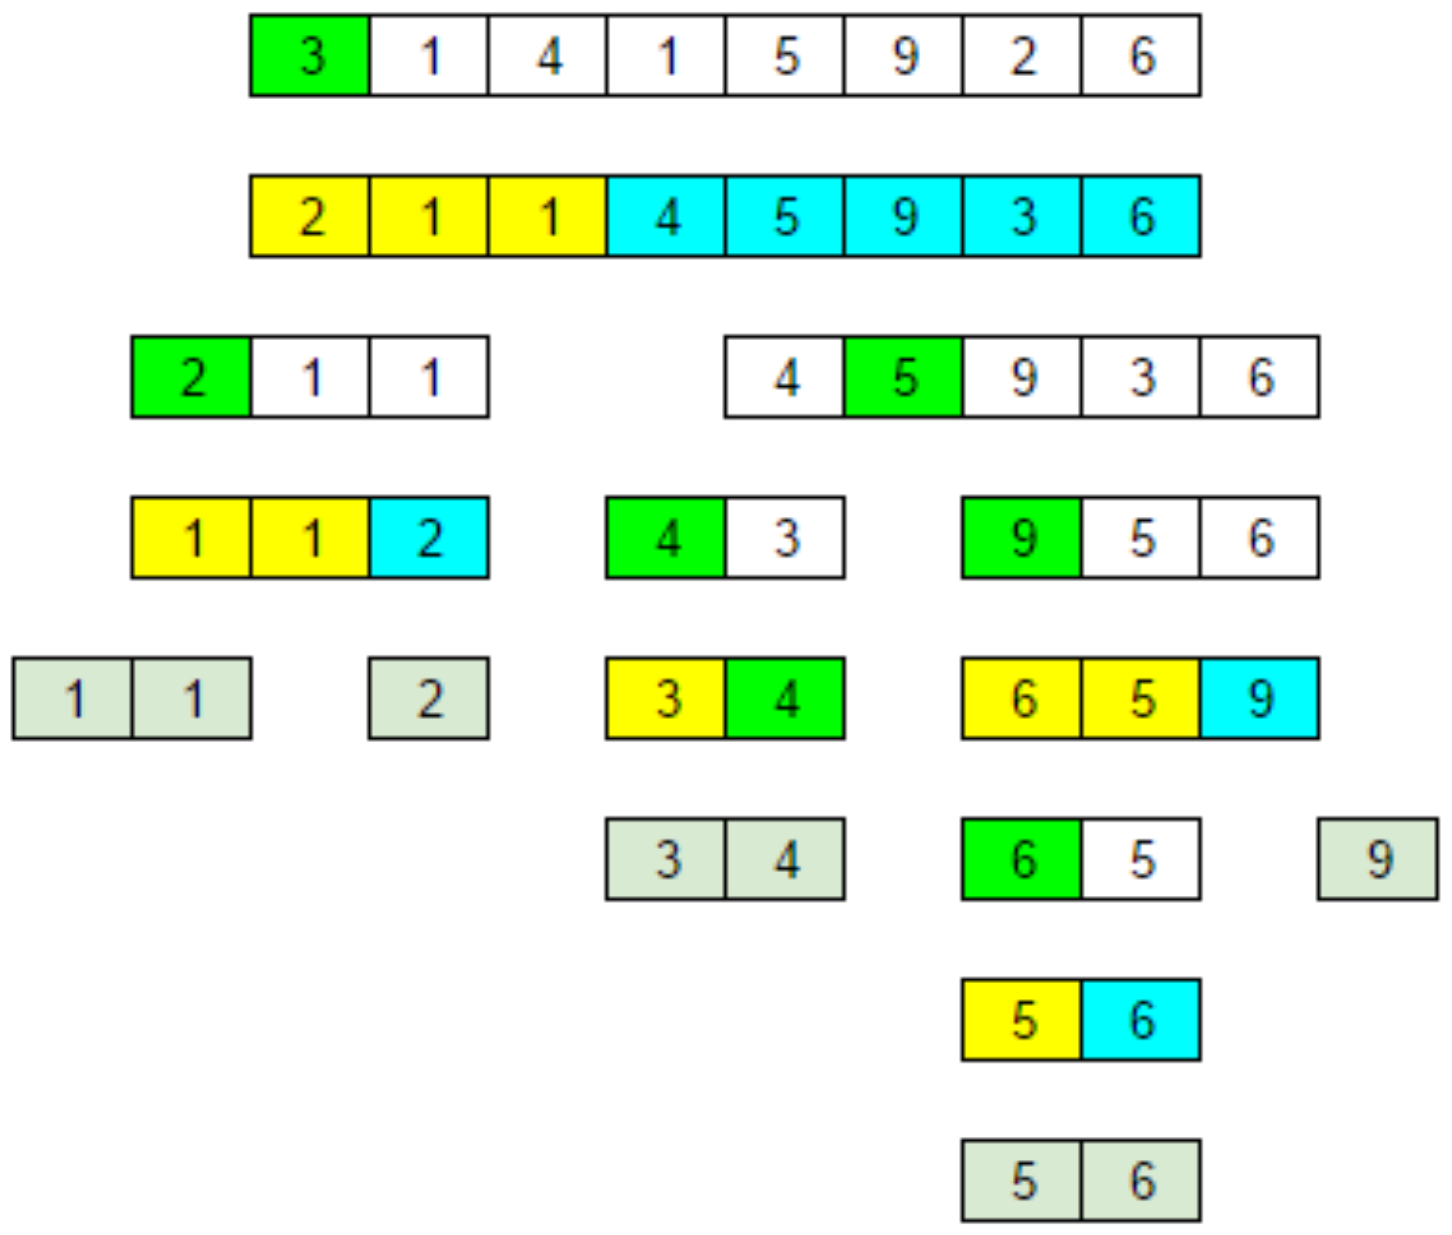
\includegraphics[width=\textwidth]{qsort.png}
			\end{column}
			\begin{column}{0.5\textwidth}
				\begin{itemize}
					\item $O(n * log(n))$, вырождается до $O(n^2)$
					\item Неустойчива
					\item Требует $O(n * log(n))$ дополнительной памяти
					\item Самый быстрый на практике алгоритм сортировки, используется в стандартных библиотеках
					\item Легко пишется (но тяжело отлаживается)
				\end{itemize}
			\end{column}
		\end{columns}
	\end{frame}

	\begin{frame}[fragile]
		\frametitle{Псевдокод}
		\begin{columns}
			\begin{column}{0.5\textwidth}
				\begin{minted}{text}
algorithm quicksort(A, lo, hi) is
    if lo < hi then
        p := partition(A, lo, hi)
        quicksort(A, lo, p – 1)
        quicksort(A, p + 1, hi)
				\end{minted}
			\end{column}
			\begin{column}{0.5\textwidth}
				\begin{minted}{text}
algorithm partition(A, lo, hi) is
    pivot := A[hi]
    i := lo  
    for j := lo to hi – 1 do
        if A[j] ≤ pivot then
            swap A[i] with A[j]
            i := i + 1
    swap A[i] with A[hi]
    return i
				\end{minted}
			\end{column}
		\end{columns}

		\vspace{5mm}
		Нерекурсивная реализация --- через стек, в котором хранятся границы сортируемых кусков массива
	\end{frame}

	\begin{frame}
		\frametitle{Сортировка кучей (пирамидальная, heapsort)}
		\begin{columns}
			\begin{column}{0.5\textwidth}
				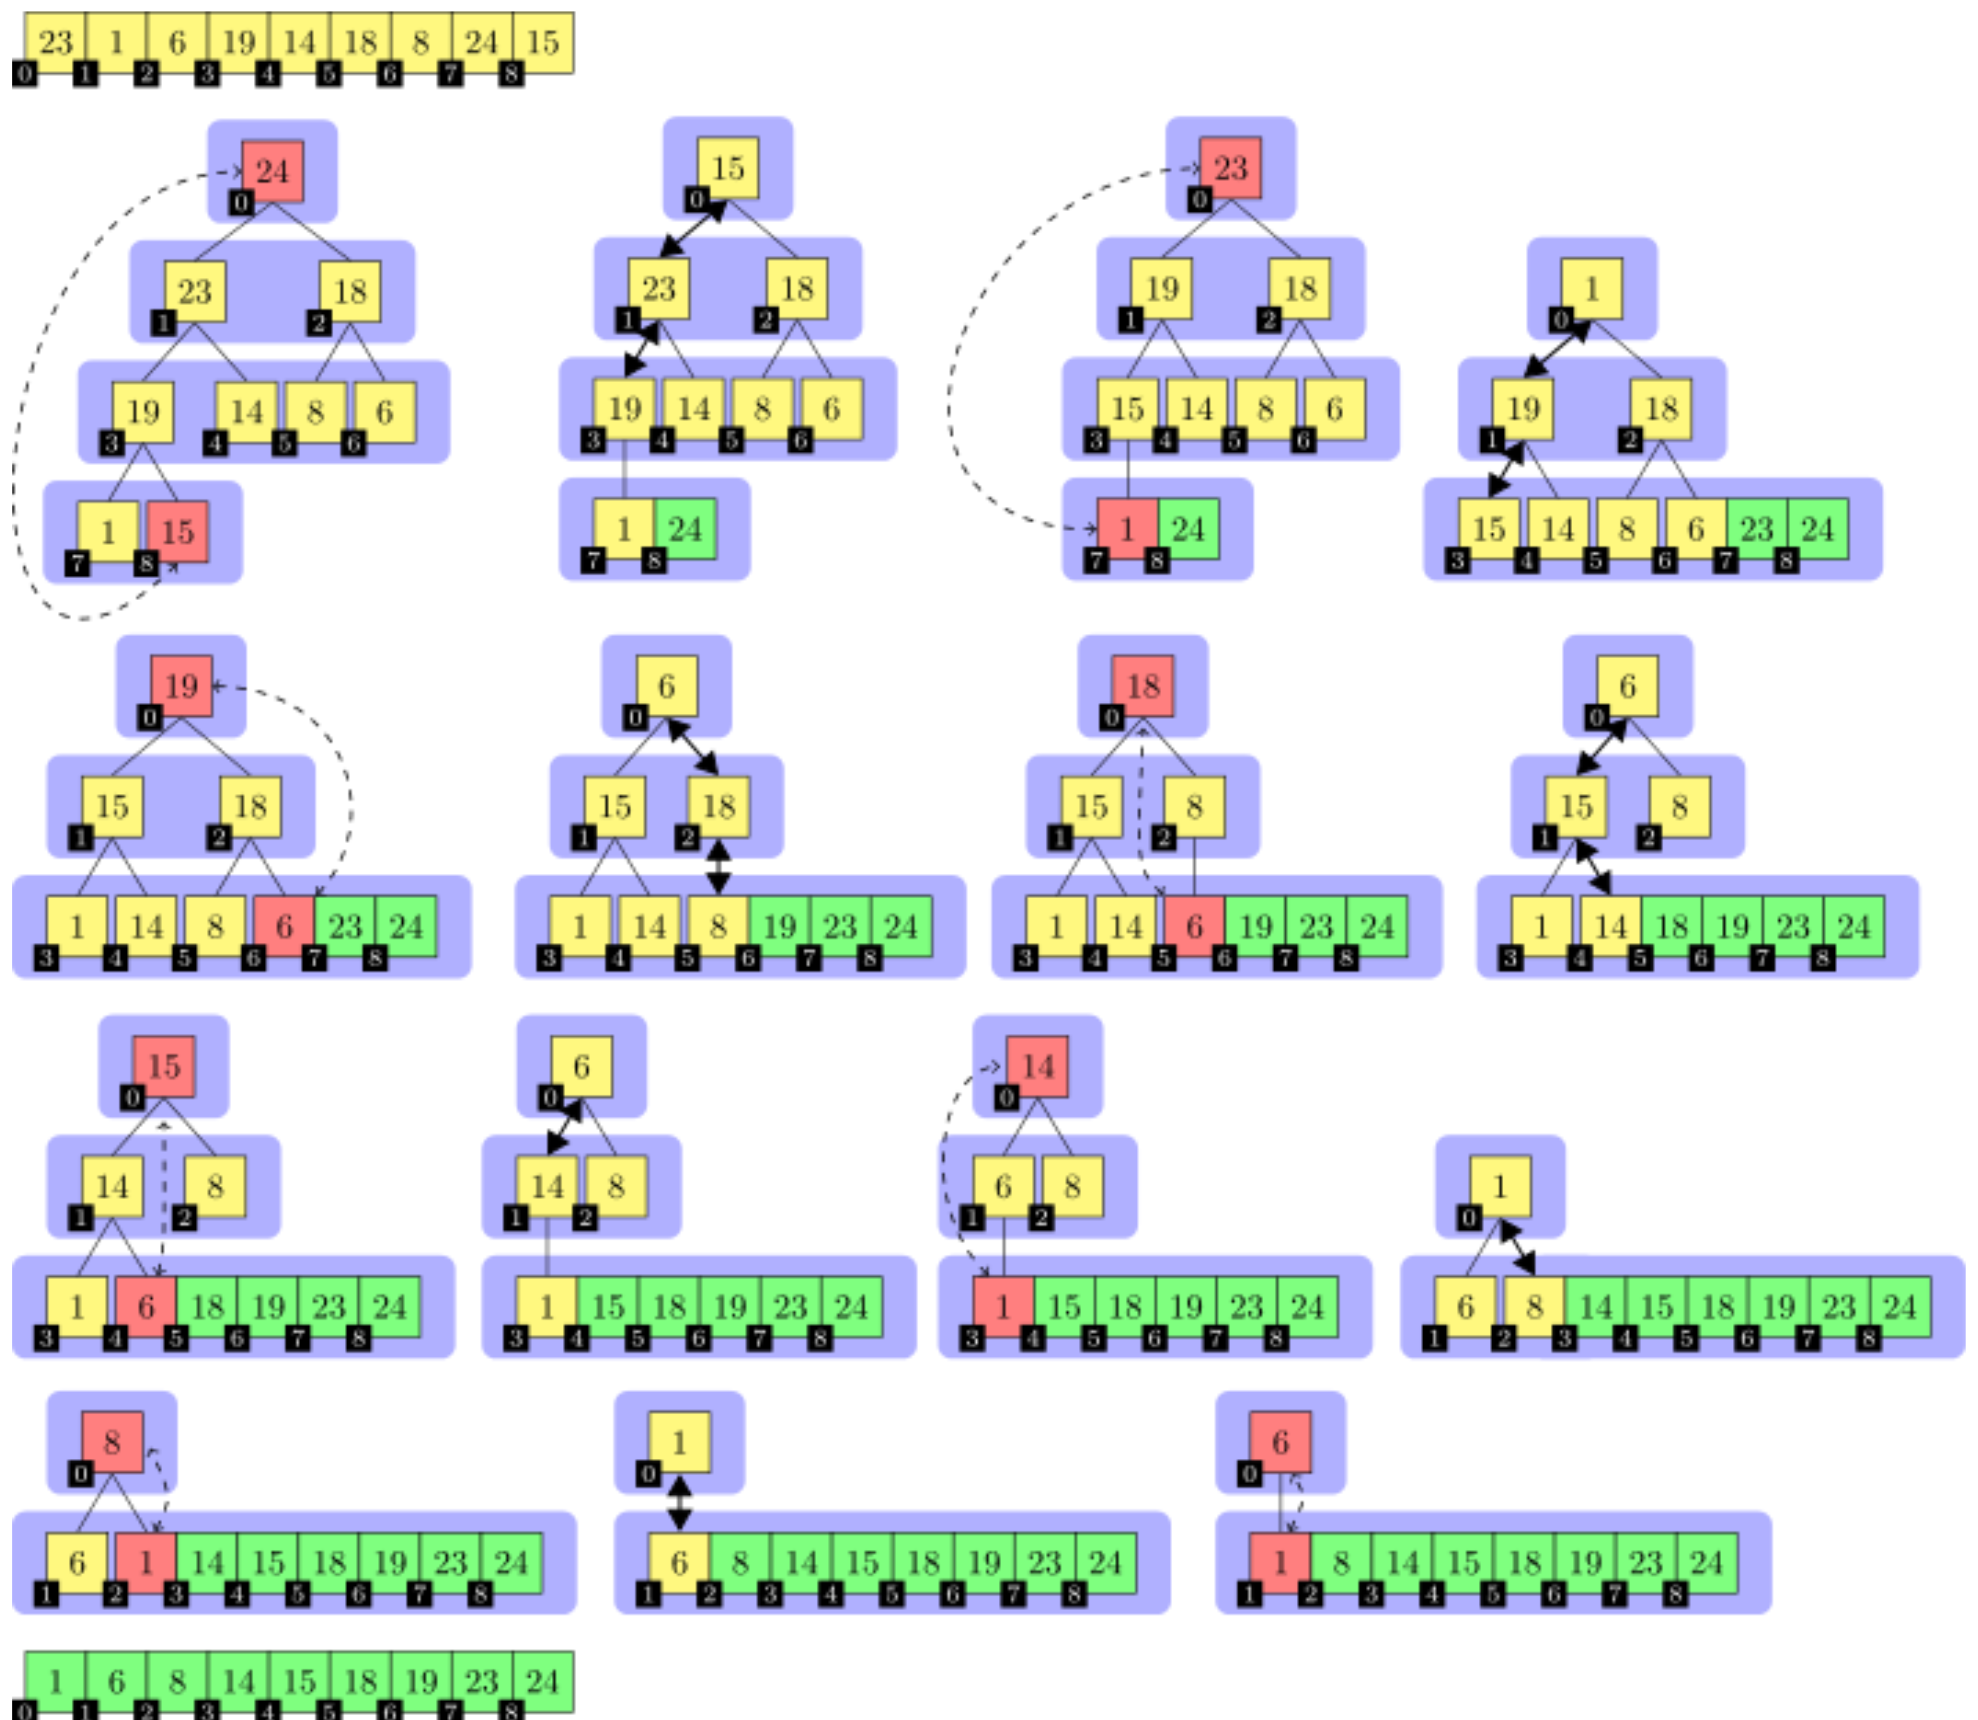
\includegraphics[width=\textwidth]{heapsort.png}
			\end{column}
			\begin{column}{0.5\textwidth}
				\begin{itemize}
					\item $O(n * log(n))$, не вырождается
					\item Не требует дополнительной памяти
					\item Неустойчива
					\item Требует произвольного доступа к памяти
					\item Относительно сложна в реализации
					\item url{https://www.ee.ryerson.ca/~courses/coe428/sorting/heapsort.html}
				\end{itemize}
			\end{column}
		\end{columns}
	\end{frame}

	\begin{frame}
		\frametitle{Сортировка слиянием (mergesort)}
		\begin{columns}
			\begin{column}{0.45\textwidth}
				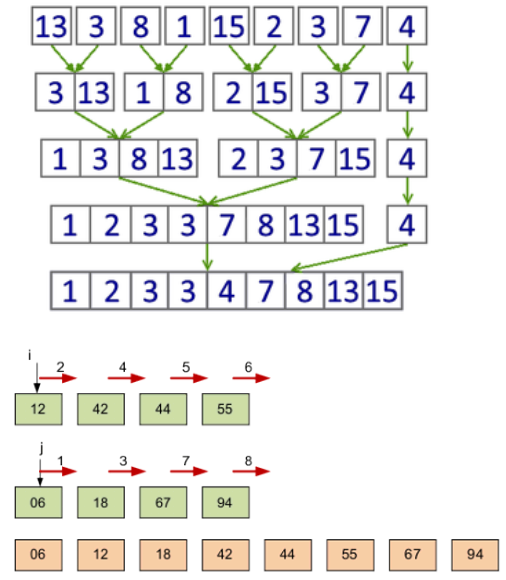
\includegraphics[width=\textwidth]{mergesort.png}
			\end{column}
			\begin{column}{0.55\textwidth}
				\begin{itemize}
					\item $O(n * log(n))$, не вырождается
					\item Устойчива
					\item Внешняя (подходит для больших данных, не помещающихся в память)
					\item \url{http://www.ee.ryerson.ca/~courses/coe428/sorting/mergesort.html}
				\end{itemize}
			\end{column}
		\end{columns}
	\end{frame}

	\begin{frame}
		\frametitle{Двоичный поиск}
		\begin{columns}
			\begin{column}{0.5\textwidth}
				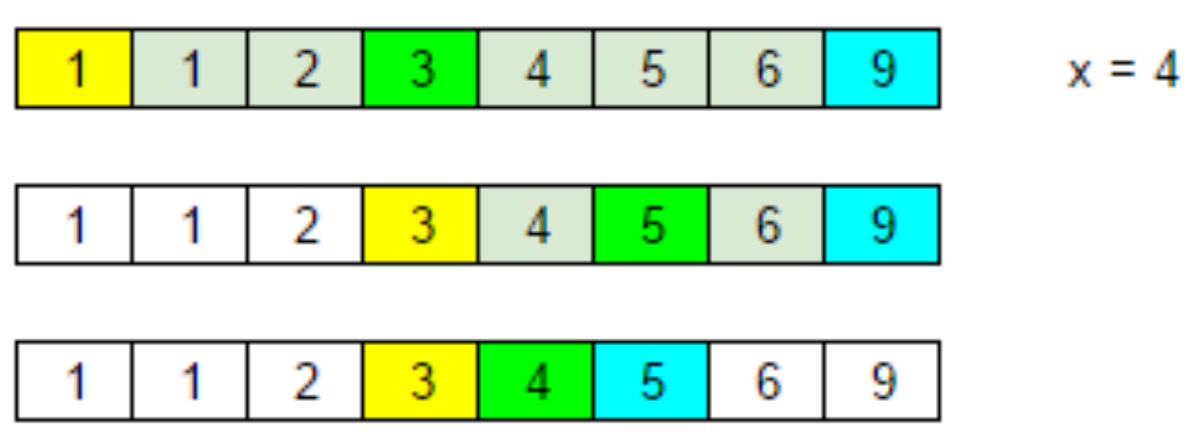
\includegraphics[width=\textwidth]{binSearch.png}
			\end{column}
			\begin{column}{0.5\textwidth}
				\begin{itemize}
					\item Находит элемент в массиве за $O(log(n))$
					\item Легко напутать с индексами и уйти в бесконечный цикл
				\end{itemize}
			\end{column}
		\end{columns}
	\end{frame}

\end{document}